\documentclass[11pt,notes=hide,aspectratio=169,mathserif]{beamer}

% PACKAGES
\usepackage{graphics}  % Support for images/figures
\usepackage{graphicx}  % Includes the \resizebox command
\usepackage{tikz}      % For flowcharts
\usetikzlibrary{arrows.meta, positioning} % Libraries for TikZ


\usepackage{url}	   % Includes \urldef and \url commands
\usepackage{natbib}
\usepackage{bibentry}  % Includes the \nobibliography command
\usepackage{verbatim}  %Supports comments
\usepackage{booktabs} %Supports \toprule, \bottomrule, etc in tables
\usepackage{etoolbox}  %Supports toggle commands
\usepackage{datetime}
\usepackage{bm}	%Supports bold math \bm
%the LaTeX standard:
\usepackage{cmbright}
\setbeamerfont{frametitle}{family=\fontfamily{cmbr}\selectfont,size=\Large}
\fontencoding{OT1}\fontfamily{cmbr}\selectfont

% PACKAGES (that should already be included by your LyX document settings)
\usepackage{amsfonts}  % Lots of stuff, including \mathbb 
\usepackage{amsmath}   % Standard math package
\usepackage{amsthm}    % Includes the comment functions
\usepackage{subcaption}

% CUSTOM DEFINITIONS
\def\newblock{} %Get beamer to cooperate with BibTeX
\linespread{1.2}

% IDENTIFYING INFORMATION
\title[class]{ECON 326: Economics of Developing Countries \\ TA Session 4}
\author[vaidehi's class ]{Vaidehi Parameswaran (Northwestern Econ)}
\date{\monthname[\the\month] \the\year}

% THEMATIC OPTIONS
%\setbeamercovered{transparent}
\usetheme{metropolis}
\definecolor{mycolor}{RGB}{0,153,153} % define cyan colour
\setbeamercolor{frametitle}{bg=mycolor, fg=white} % Frame title color
\setbeamercolor{title separator}{fg=mycolor} 
\setbeamercolor{progress bar}{fg=mycolor} 
\beamertemplatenavigationsymbolsempty
\setbeamertemplate{footline}[frame number]{}
\setbeamertemplate{itemize item}{\small\raisebox{1pt}{\textcolor{mycolor}{$\blacktriangleright$}}}
\setbeamertemplate{itemize subitem}{\footnotesize\raisebox{1pt}{\textcolor{mycolor}{$\triangleright$}}}
\setbeamertemplate{itemize subsubitem}{\tiny\raisebox{1pt}{\textcolor{mycolor}{$\triangleright$}}}

% BACKUP SLIDE NUMBERING
\usepackage{appendixnumberbeamer}

\begin{document}

%---------------------------------------------------------------------
\begin{frame}[plain]
\titlepage
\end{frame}
%---------------------------------------------------------------------

%\section{Overview}

%---------------------------------------------------------------------
\begin{frame}{Today's Agenda}

\begin{itemize}
\item Benefits of Education - Duflo (2001)
\item Problem Set 2 - Some Pointers 
\end{itemize}
\end{frame}
%---------------------------------------------------------------------



\section*{\href{https://www.aeaweb.org/articles?id=10.1257/0002828041302109}{\textcolor{blue}{Duflo (2001)}} \\[5mm] 
\textnormal{\small{Schooling and Labour Market Consequences of School Construction in Indonesia}}}

%---------------------------------------------------------------------
\begin{frame}{Overview}
\begin{itemize}
\item A very influential paper that uses non-experimental methods 
\item Evaluates the impact of a large school construction program in Indonesia
\item This was not an RCT, but a quasi-experimental design
\item The author uses a difference-in-difference strategy to estimate the impact of the program
\item Combined with an IV strategy to estimate returns to school
\item Findings are consistent with other papers (e.g., Angrist \& Krueger 1991)
\end{itemize}
\end{frame}
%---------------------------------------------------------------------

%---------------------------------------------------------------------
\begin{frame}{The Benefits of Education}
\begin{itemize}
\item Why do people send their children to school?
\begin{itemize}
    \item  Knowledge as an end in itself
    \item  Labour market: earnings, access to formal jobs, profitability of own business
    \item  Social status
    \item  Political attitudes and participation
\end{itemize}
\item  To economists, education is a form of human capital - you invest in it and get returns in the form of higher earnings (and other benefits)
\item  This is especially interesting in developing countries, where the returns to education are often higher than in developed countries
\end{itemize}
\end{frame}
%---------------------------------------------------------------------

%---------------------------------------------------------------------
\begin{frame}{Why is it hard to estimate the returns to schooling?}
\begin{itemize}
\item Mincer equation: $\ln(W) = \beta_0 + \beta_1 S + \beta_2 X + \beta_3 X^2 + \varepsilon$
\item But we know by now that correlations are not causations
\item What are possible biases? 
\begin{itemize}
\item  Selection bias: People who go to school are different from those who don't
\item  Reverse causality: People who are have higher expected potential earnings may choose to go to school 
\item  Omitted variables: There may be other factors that affect both schooling and potential earnings
\end{itemize}
\item  Ideal experiment?
\item  Can we randomly assign ``education'' to people? 
\end{itemize}
\end{frame}
%---------------------------------------------------------------------

%---------------------------------------------------------------------
\begin{frame}{Assigning an ``Instrument''}
\begin{itemize}
\item But one can randomly assign a student to a program which may increase their education 
\begin{itemize}
\item  Examples of such interventions? 
\end{itemize}
\item  Then we can exploit the effect an intervention has on education 
\begin{itemize}
\item  If the intervention has no direct effect on earnings (or other outcomes), but it does affect earnings in the data, then you can infer that it affected earnings through education alone, and hence that education affects earnings 
\end{itemize}
\item  Today's paper uses this insight 
\item  Then we can apply this technique in a non-experimental setting
\end{itemize}
\end{frame}
%---------------------------------------------------------------------

%---------------------------------------------------------------------
\begin{frame}{Sekolah Dasar INPRES}
\begin{itemize}
\item In 1973, Indonesian government prioritised ``equity'' across provinces
\item Launched a large school construction program
\item Between 1973-1974 and 1978-1979, 61,807 schools were built
\item The largest and the fastest school construction program in the world
\item Financed by oil boom revenues
\item Explicitly targeted children who were previously not enrolled in school 
    \begin{itemize}
        \item Number of schools in each district was proportional to number of children of primary school age not enrolled in 1972
    \end{itemize}
\end{itemize}
\end{frame}
%---------------------------------------------------------------------

%---------------------------------------------------------------------
\begin{frame}{Data}
\begin{itemize}
\item Intercensal survey data in 1995 
\begin{itemize}
    \item Focus on men born between 1950 and 1972
\end{itemize}   
\item Match with district-level census data and number of schools built in each district
\end{itemize}
\end{frame}
%---------------------------------------------------------------------

%---------------------------------------------------------------------
\begin{frame}{Empirical Strategy (I)}
\begin{itemize}
\item Goal: Estimate the effect of INPRES on schooling and labour market outcomes.
\item  Key idea: Children born before 1962 were 12 years or older in 1974 and were not affected by the program.
\item  So children in Indonesia belong to one of these cells:
\end{itemize}
{
\begin{table}
\scriptsize
\centering
\begin{tabular}{|c|c|c|}
\hline
    & \multicolumn{2}{|c|}{\textbf{INPRES Intensity in Region of Birth}}  \\
    \hline
    \textbf{Cohorts} & \textbf{High} & \textbf{Low}  \\
\hline 
\textbf{(A)} Aged 2-6 in 1974:  & \rule{0pt}{15pt}  \textcolor{blue}{High Exposure to INPRES} & \rule{0pt}{15pt} \textcolor{gray}{Low Exposure to INPRES} \\
\hline
\textbf{(B)} Aged 12-17 in 1974:  & \rule{0pt}{15pt} \textcolor{gray}{Low Exposure to INPRES} & \rule{0pt}{15pt} \textcolor{gray}{Low Exposure to INPRES} \\
\hline
\end{tabular}
\end{table}
}
\end{frame}
%---------------------------------------------------------------------

%---------------------------------------------------------------------
\begin{frame}{Empirical Strategy (II)}
\begin{table}
\scriptsize
\centering
\begin{tabular}{|c|c|c|}
\hline
    & \multicolumn{2}{|c|}{\textbf{INPRES Intensity in Region of Birth}}  \\
    \hline
    \textbf{Cohorts} & \textbf{High} & \textbf{Low}  \\
\hline 
\textbf{(A)} Aged 2-6 in 1974:  & \rule{0pt}{15pt}  \textcolor{blue}{High Exposure to INPRES} & \rule{0pt}{15pt} \textcolor{gray}{Low Exposure to INPRES} \\
\hline
\textbf{(B)} Aged 12-17 in 1974:  & \rule{0pt}{15pt} \textcolor{gray}{Low Exposure to INPRES} & \rule{0pt}{15pt} \textcolor{gray}{Low Exposure to INPRES} \\
\hline
\end{tabular}
\end{table}

\begin{itemize}
    \item  Naive approach: Compare cohorts A and B to estimate the effect of INPRES
    \item  But this can underestimate the actual effects of INPRES:
    \begin{itemize}
        \item  Only those in high-intensity regions get the full benefits of the policy
    \end{itemize} 
    \item  And it's hard to argue that cohorts A and B \textit{only} differ in exposure to INPRES
    \begin{itemize}
        \item  If Indonesia is experiencing growth over time, we expect cohort A to do better, regardless of whether INPRES is implemented
    \end{itemize}
\end{itemize}
\end{frame}
%---------------------------------------------------------------------

%---------------------------------------------------------------------
\begin{frame}{Empirical Strategy (III)}
\begin{table}
\scriptsize
\centering
\begin{tabular}{|c|c|c|}
\hline
    & \multicolumn{2}{|c|}{\textbf{INPRES Intensity in Region of Birth}}  \\
    \hline
    \textbf{Cohorts} & \textbf{High} & \textbf{Low}  \\
\hline 
\textbf{(A)} Aged 2-6 in 1974:  & \rule{0pt}{15pt}  \textcolor{blue}{High Exposure to INPRES} & \rule{0pt}{15pt} \textcolor{gray}{Low Exposure to INPRES} \\
\hline
\textbf{(B)} Aged 12-17 in 1974:  & \rule{0pt}{15pt} \textcolor{gray}{Low Exposure to INPRES} & \rule{0pt}{15pt} \textcolor{gray}{Low Exposure to INPRES} \\
\hline
\end{tabular}
\end{table}

\begin{itemize}
    \item  Another naive approach: Compare high vs low intensity regions 
    \item  But this is misleading as well:
    \begin{itemize}
        \item  INPRES targeted regions that were worse off to begin with
        \item  So we expect people in high-intensity regions to do worse, regardless of INPRES
    \end{itemize} 
\end{itemize}
\end{frame}
%---------------------------------------------------------------------

%---------------------------------------------------------------------
\begin{frame}{Empirical Strategy (IV)}
\begin{table}
\scriptsize
\centering
\begin{tabular}{|c|c|c|}
\hline
    & \multicolumn{2}{|c|}{\textbf{INPRES Intensity in Region of Birth}}  \\
    \hline
    \textbf{Cohorts} & \textbf{High} & \textbf{Low}  \\
\hline 
\textbf{(A)} Aged 2-6 in 1974:  & \rule{0pt}{15pt}  \textcolor{blue}{High Exposure to INPRES} & \rule{0pt}{15pt} \textcolor{gray}{Low Exposure to INPRES} \\
\hline
\textbf{(B)} Aged 12-17 in 1974:  & \rule{0pt}{15pt} \textcolor{gray}{Low Exposure to INPRES} & \rule{0pt}{15pt} \textcolor{gray}{Low Exposure to INPRES} \\
\hline
\end{tabular}
\end{table}

\begin{itemize}
    \item  Solution: Use both the variation from cohorts and the variation from intensity and combine the two naive approaches
    \item  For each region, we compare the outcomes of cohort A relative to cohort B
    \item  Then we compare the changes in outcomes between high and low intensity regions
    \item  What is the key assumption for this to work?
    \begin{itemize}
        \item Factors that make high and low intensity regions different affect each cohort identically 
    \end{itemize} 
\end{itemize}
\end{frame}
%---------------------------------------------------------------------

%---------------------------------------------------------------------
\begin{frame}{Empirical Strategy (V)}
\begin{itemize}
    \item This was a classic example of a difference-in-difference strategy
    \item  The key identifying assumption: \textbf{Parallel Trends Assumption}
    \begin{itemize}
        \item   In the absence of INPRES, the outcomes of cohorts A and B in high and low intensity regions would have evolved in the same way
    \end{itemize}
\end{itemize}
\begin{figure}
    \centering
    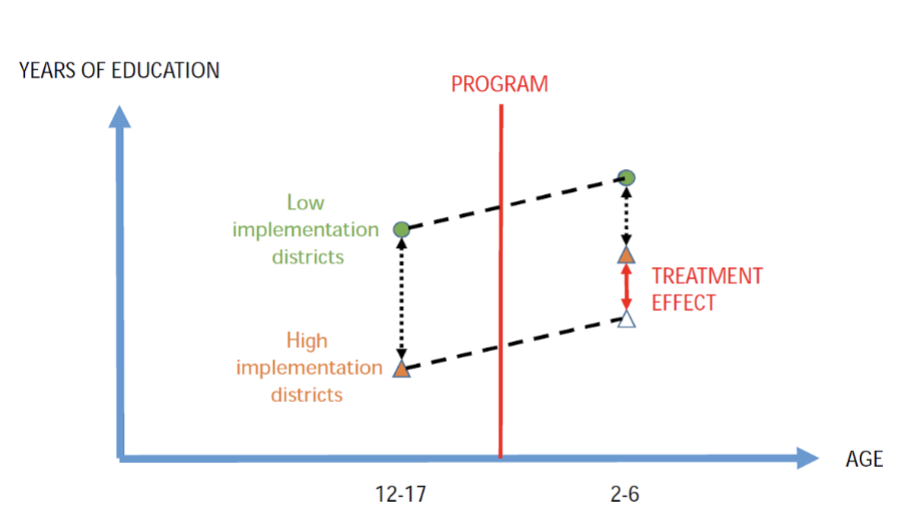
\includegraphics[width=0.5\textwidth]{inputs/diagram1.png}
\end{figure}
\end{frame}
%---------------------------------------------------------------------

%---------------------------------------------------------------------
\begin{frame}{Empirical Strategy (VI)}
\begin{itemize}
    \item Fundamentally untestable assumption
    \item  But we can verify its plausibility by looking at pre-trends 
    \item Compare a new placebo cohort (C) to cohort B
    \begin{itemize}
        \item  If the outcomes of cohorts B and C evolve the same way, then we have suggestive evidence that there were no different intergenerational effects by region 
    \end{itemize}
\end{itemize}
{
\begin{figure}
    \centering
    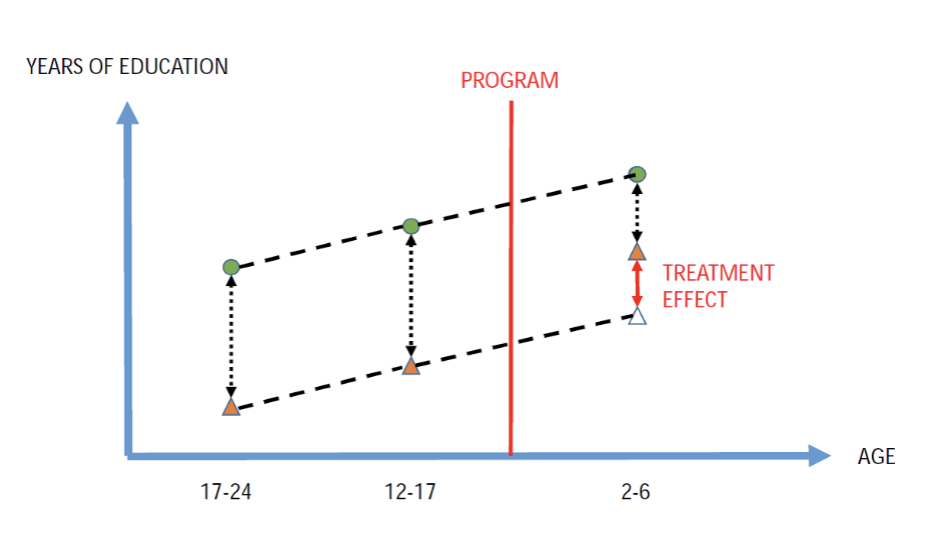
\includegraphics[width=0.5\textwidth]{inputs/diagram2.png}
\end{figure}
}
\end{frame}
%---------------------------------------------------------------------

%---------------------------------------------------------------------
\begin{frame}{Empirical Strategy (Regression)}
\begin{itemize}
    \item Let $P_j$ be program intensity in region (number of schools per 1,000 children)
    \item Let $T_i$ be an indicator for cohort A (the young cohort) 
    \item Let $C_j$ be a vector of region characteristics 
    \item Duflo (2001) estimates the effect of the program on schooling ($S_{ijk}$) and earnings $y_{ijk}$ of individual $i$ born in region $j$ in year $k$ using the following regression
\end{itemize}
\begin{align*}
    S_{ijk} &= c_1 + \alpha_{1j} + \beta_{1k} + \gamma_1 T_i * P_j + \delta_1 T_i * C_j + \epsilon_{ijk} \\
    y_{ijk} &= c_2 + \alpha_{2j} + \beta_{2k} + \gamma_2 T_i * P_j + \delta_2 T_i * C_j + \nu_{ijk}
\end{align*}
\end{frame}
%---------------------------------------------------------------------

%---------------------------------------------------------------------
\begin{frame}{Empirical Strategy (IV)}
\begin{itemize}
    \item First stage: 
    \begin{equation}
        S_{ijk} = c_1 + \alpha_{1j} + \beta_{1k} + \gamma_1 T_i * P_j + \delta_1 T_i * C_j + \epsilon_{ijk}
    \end{equation}
    \item Reduced form: 
    \begin{equation}
        y_{ijk} = c_2 + \alpha_{2j} + \beta_{2k} + \gamma_2 T_i * P_j + \delta_2 T_i * C_j + \nu_{ijk}
    \end{equation}
    \item Second stage:
    \begin{equation}
        y_{ijk} = c + \alpha_{j} + \beta_{k} + b \hat{S}_{ijk} + \delta T_i * C_j + \nu_{ijk}
    \end{equation}
    \item Coefficient of interest:
    \begin{equation}
        \hat{b} = \frac{\hat{\gamma_2}}{\hat{\gamma_1}}
    \end{equation}
\end{itemize}
\end{frame}
%---------------------------------------------------------------------

%---------------------------------------------------------------------
\begin{frame}{Results (I)}
\begin{itemize}
    \item These are the key results from the diff-in-diff strategy
    \item  INPRES raises schooling by 0.12 years and wages by 0.026 log points ($\sim 2.6\%$)
\end{itemize}
\begin{figure}
    \centering
    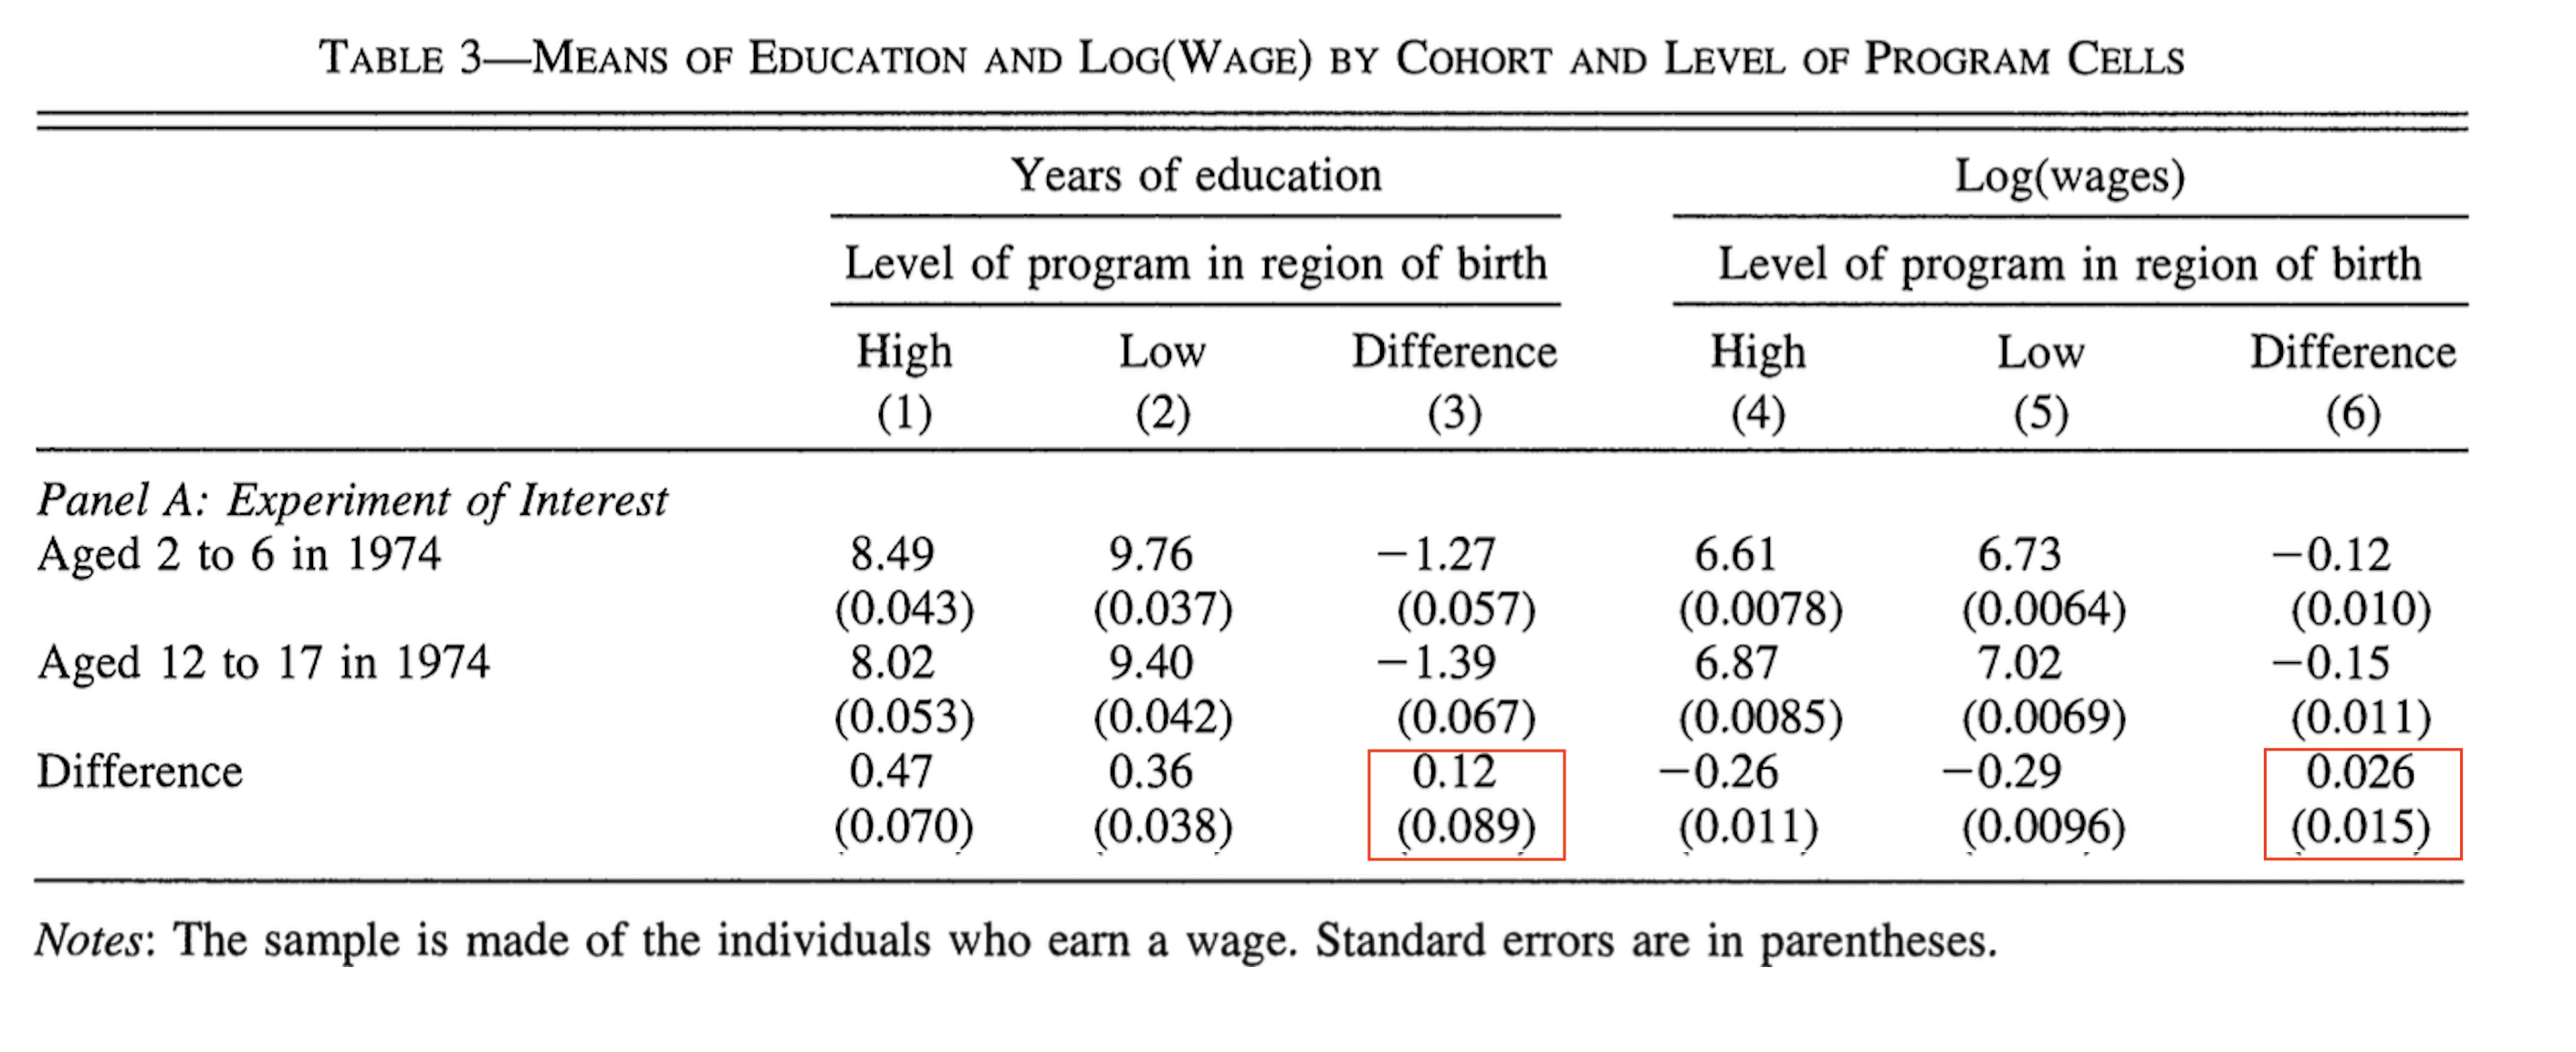
\includegraphics[width=\textwidth]{inputs/Table3a.png}
\end{figure}
\end{frame}
%---------------------------------------------------------------------

%---------------------------------------------------------------------
\begin{frame}{Results (II)}
\begin{itemize}
    \item Do we believe that INPRES \textit{only} affects wages through education?
    \begin{itemize}
        \item  If so, these results imply huge returns to education (over 20\%!)
        \item  To see this, take the ratio of both effects above: $\frac{2.6\%}{0.12}$
    \end{itemize}
\end{itemize}
\begin{figure}
    \centering
    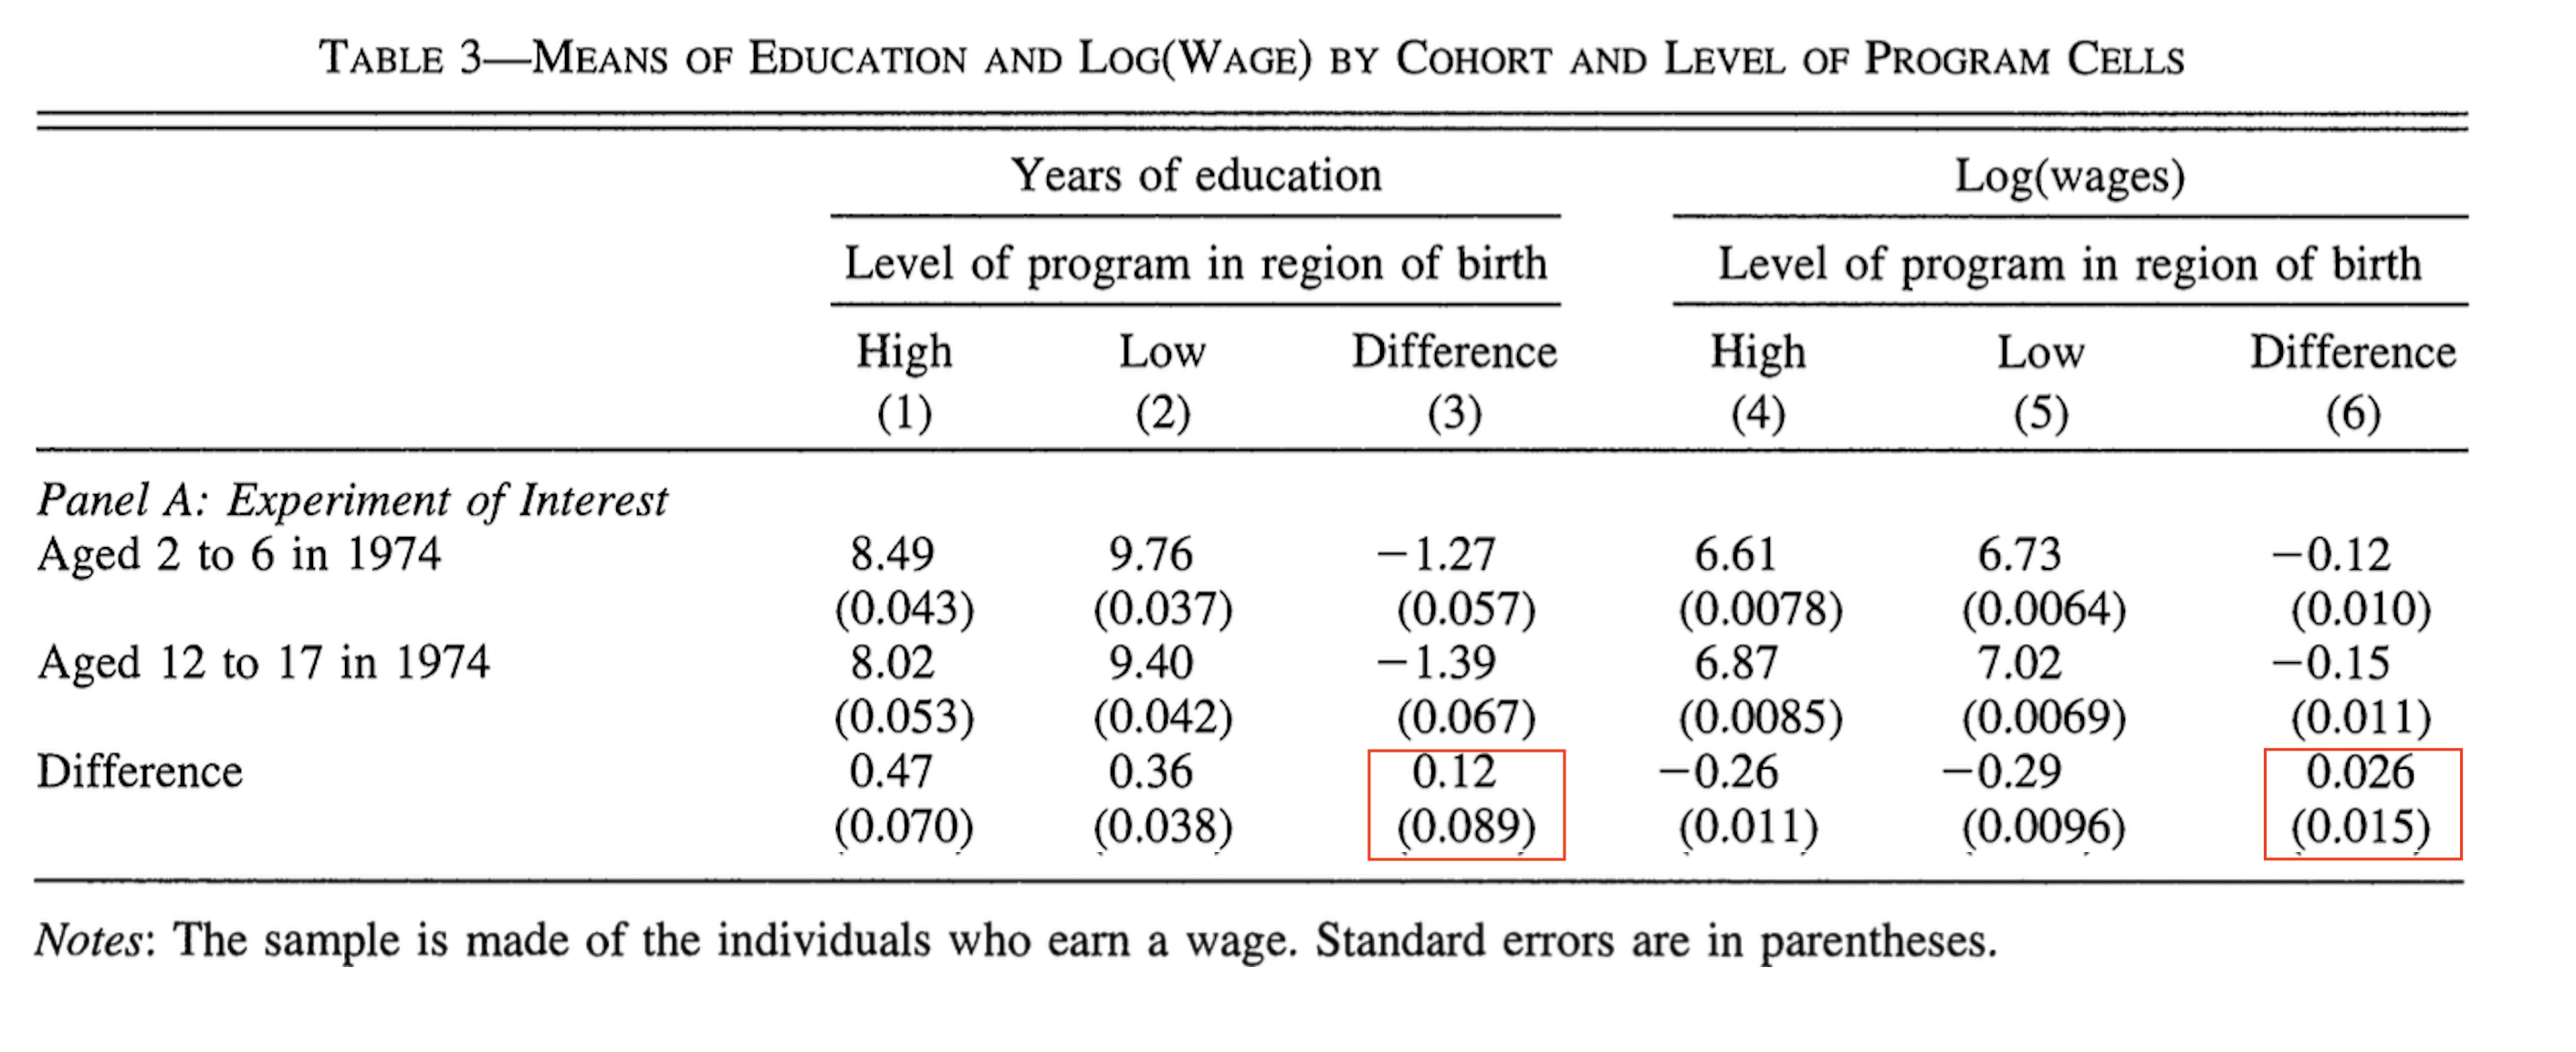
\includegraphics[width=\textwidth]{inputs/Table3a.png}
\end{figure}
\end{frame}
%---------------------------------------------------------------------

%---------------------------------------------------------------------
\begin{frame}{Results (III)}
\begin{itemize}
\item More formally: within regions, exposure to INPRES can be used as an IV
\begin{itemize}
    \item The first stage of the IV is the left panel of the table below
    \item And the right panel is its reduced form
\end{itemize}
\end{itemize}
\begin{figure}
    \centering
    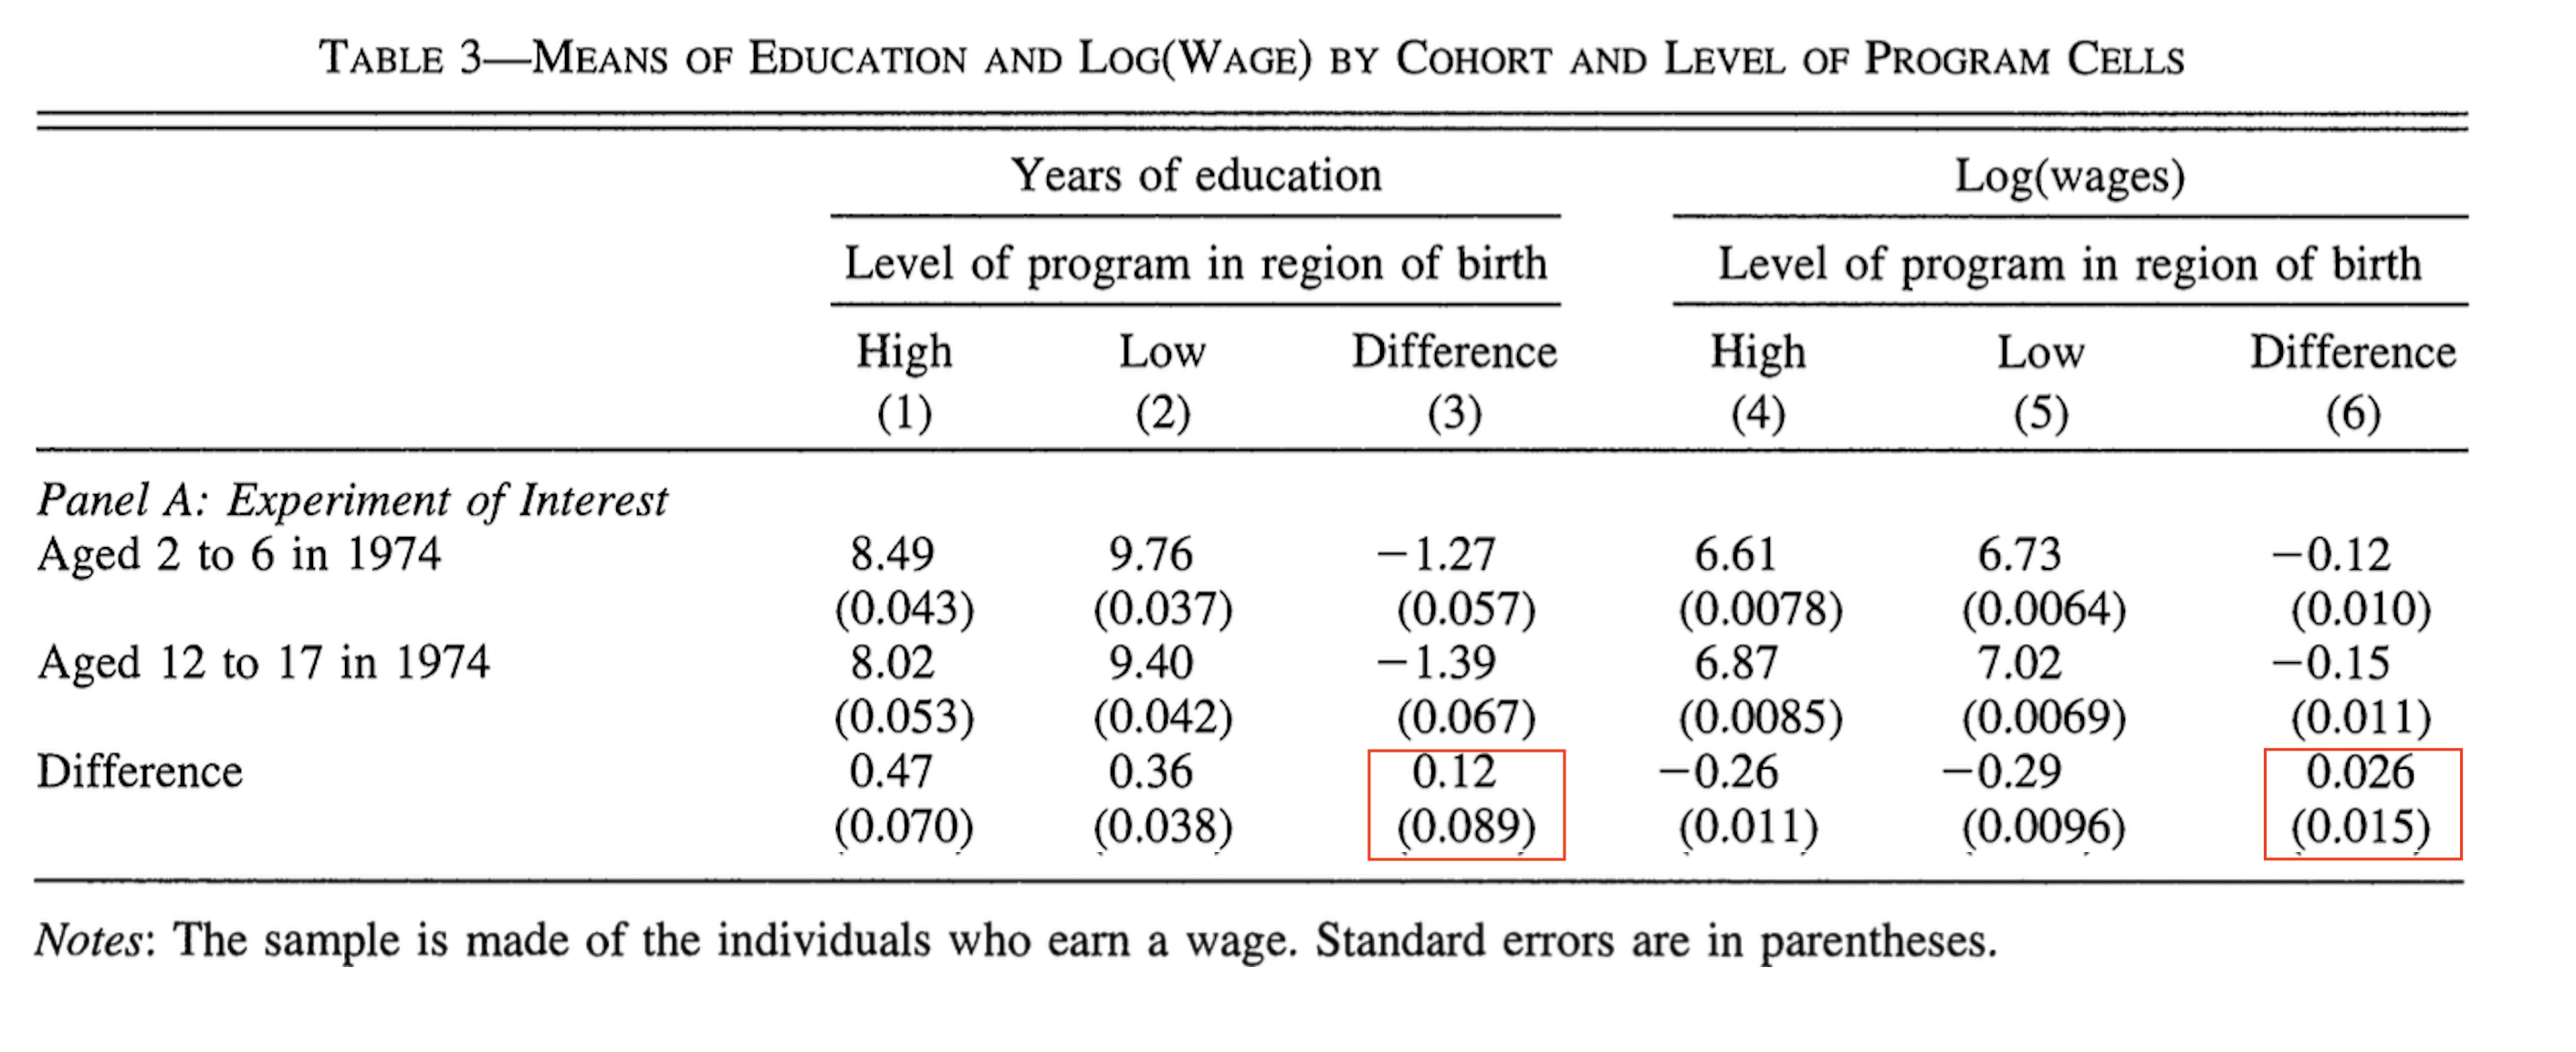
\includegraphics[width=\textwidth]{inputs/Table3a.png}
\end{figure}
\end{frame}
%---------------------------------------------------------------------

%---------------------------------------------------------------------
\begin{frame}{Results (IV)}
\begin{itemize}
\item But we have an \textbf{IV relevance} problem
\item The effect of INPRES on schooling lacks significance (coef. $\sim$ std. error) 
\begin{itemize}
    \item To address this, need to move towards a more sophisticated estimation strategy that is beyond the scope of today's session but is conceptually similar
\end{itemize}
\end{itemize}
\begin{figure}
    \centering
    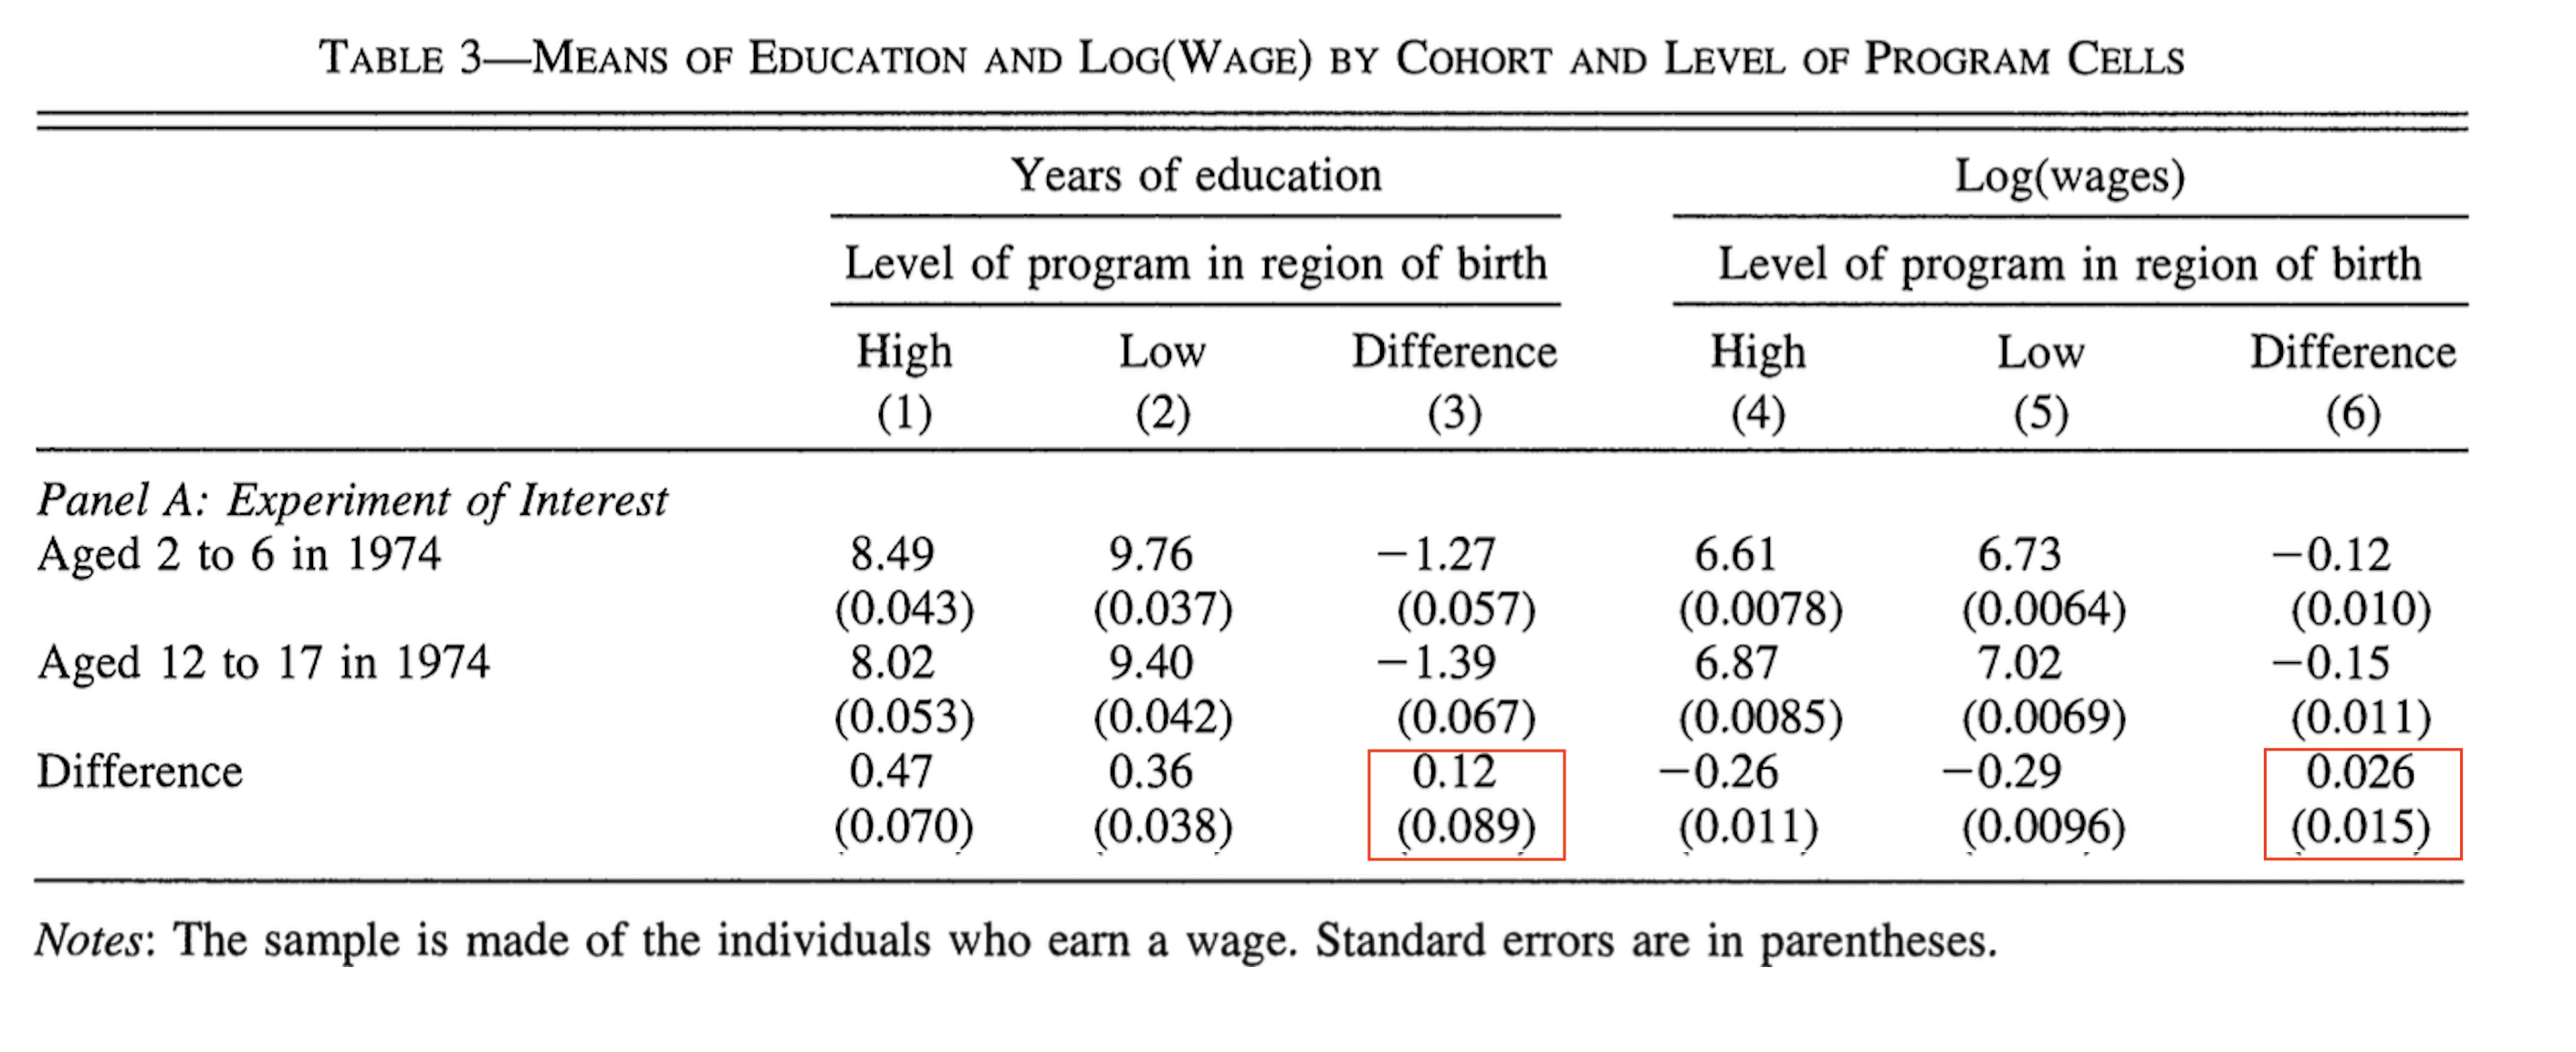
\includegraphics[width=\textwidth]{inputs/Table3a.png}
\end{figure}
\end{frame}
%---------------------------------------------------------------------

%---------------------------------------------------------------------
\begin{frame}{Results (V)}
\begin{itemize}
\item Reassuringly, non-exposed cohorts (``old'' and ``very old'') evolve similarly across high/low intensity regions
\item So we can claim that there's no evidence for differential pre-trends 
\end{itemize}
\begin{figure}
    \centering
    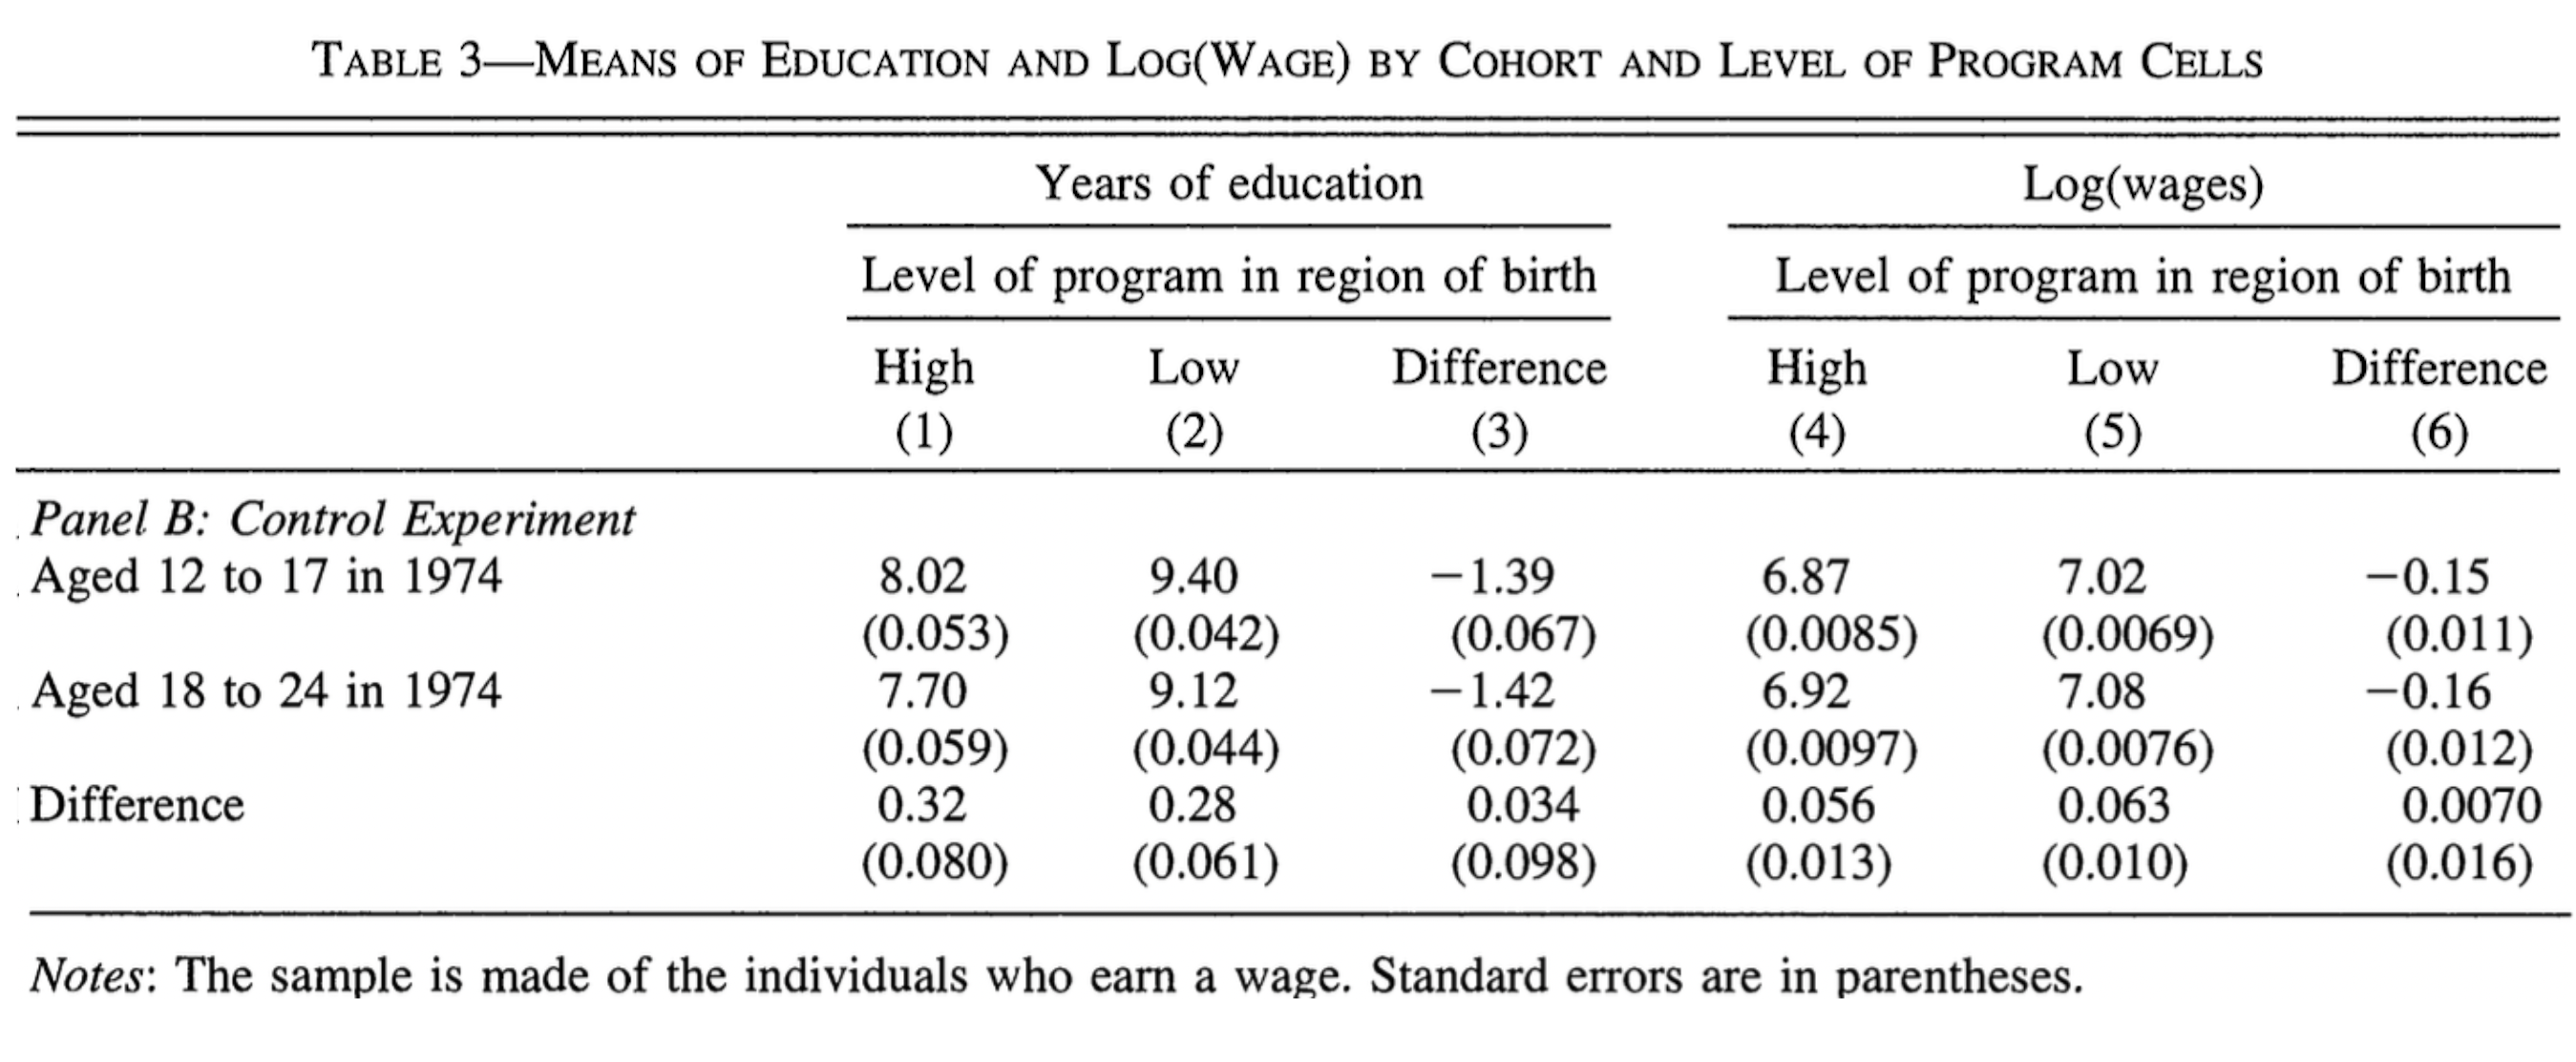
\includegraphics[width=\textwidth]{inputs/Table3b.png}
\end{figure}
\end{frame}
%---------------------------------------------------------------------

%---------------------------------------------------------------------
\begin{frame}{Results (VI)}
\begin{itemize}
\item We can extend the logic of the previous table in two ways:
\begin{itemize}
    \item Compare more than two cohorts
    \item Measure INPRES intensity continuously (as schools built per student)
\end{itemize}
\item This leads to more precise estimates of the returns to education, with smaller values that are more in line with the literature
\item The figure below illustrates how this works: we compute the correlation between INPRES intensity and schooling for each cohort
\end{itemize}
\begin{figure}
    \centering
    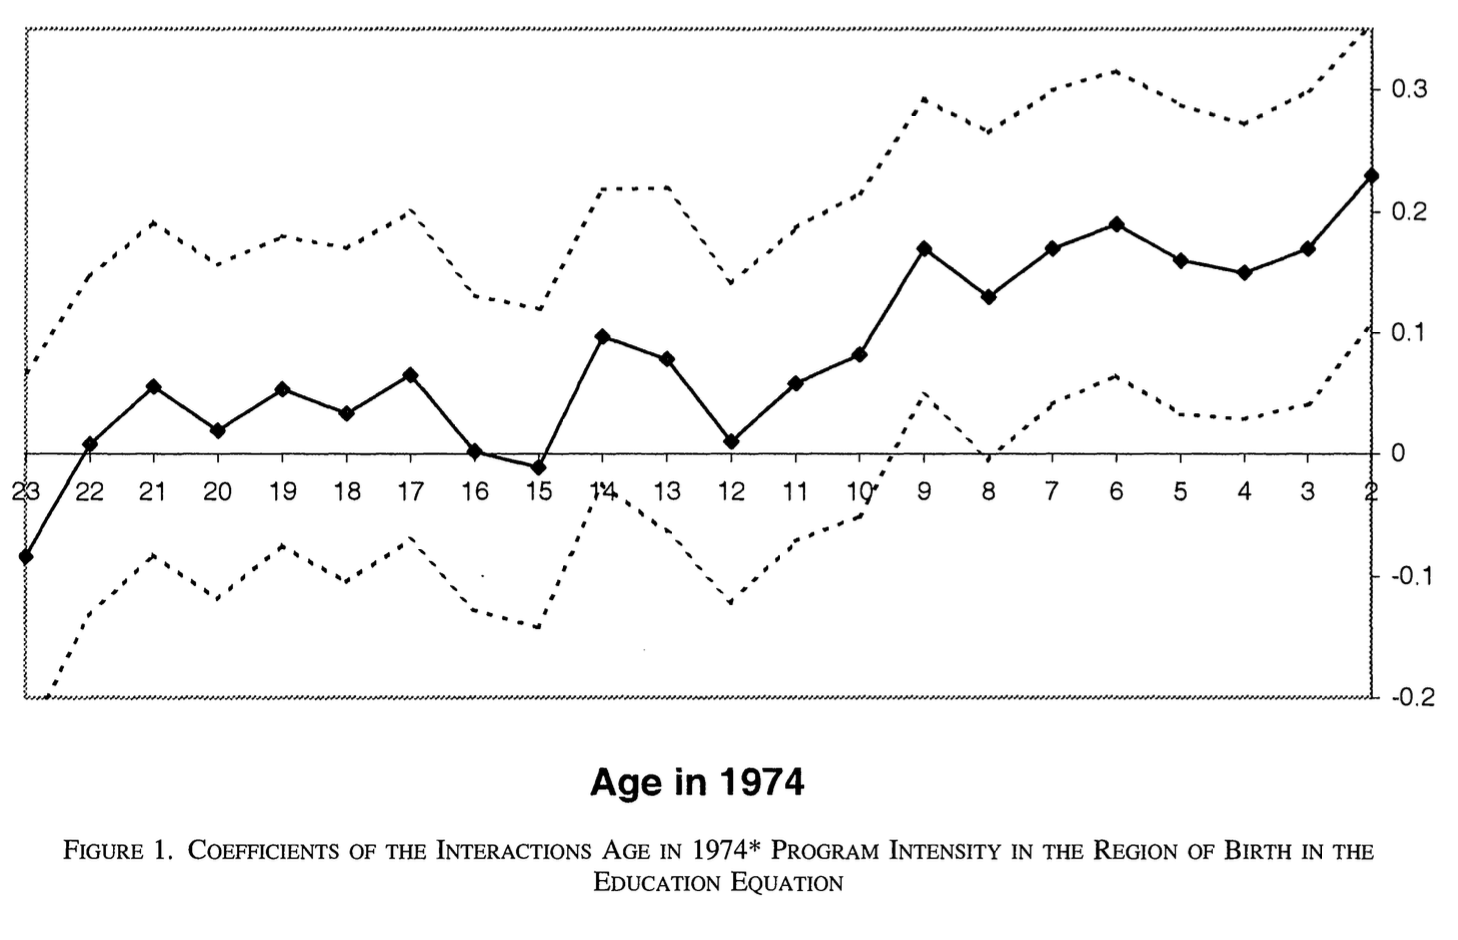
\includegraphics[width=0.4\textwidth]{inputs/Figure1.png}
\end{figure}
\end{frame}
%---------------------------------------------------------------------

%---------------------------------------------------------------------
\begin{frame}{Results (VII)}
\begin{itemize}
\item Plot of $\hat{\gamma_1}$ and $\hat{\gamma_2}$ for each cohort
\end{itemize}
\begin{figure}
    \centering
    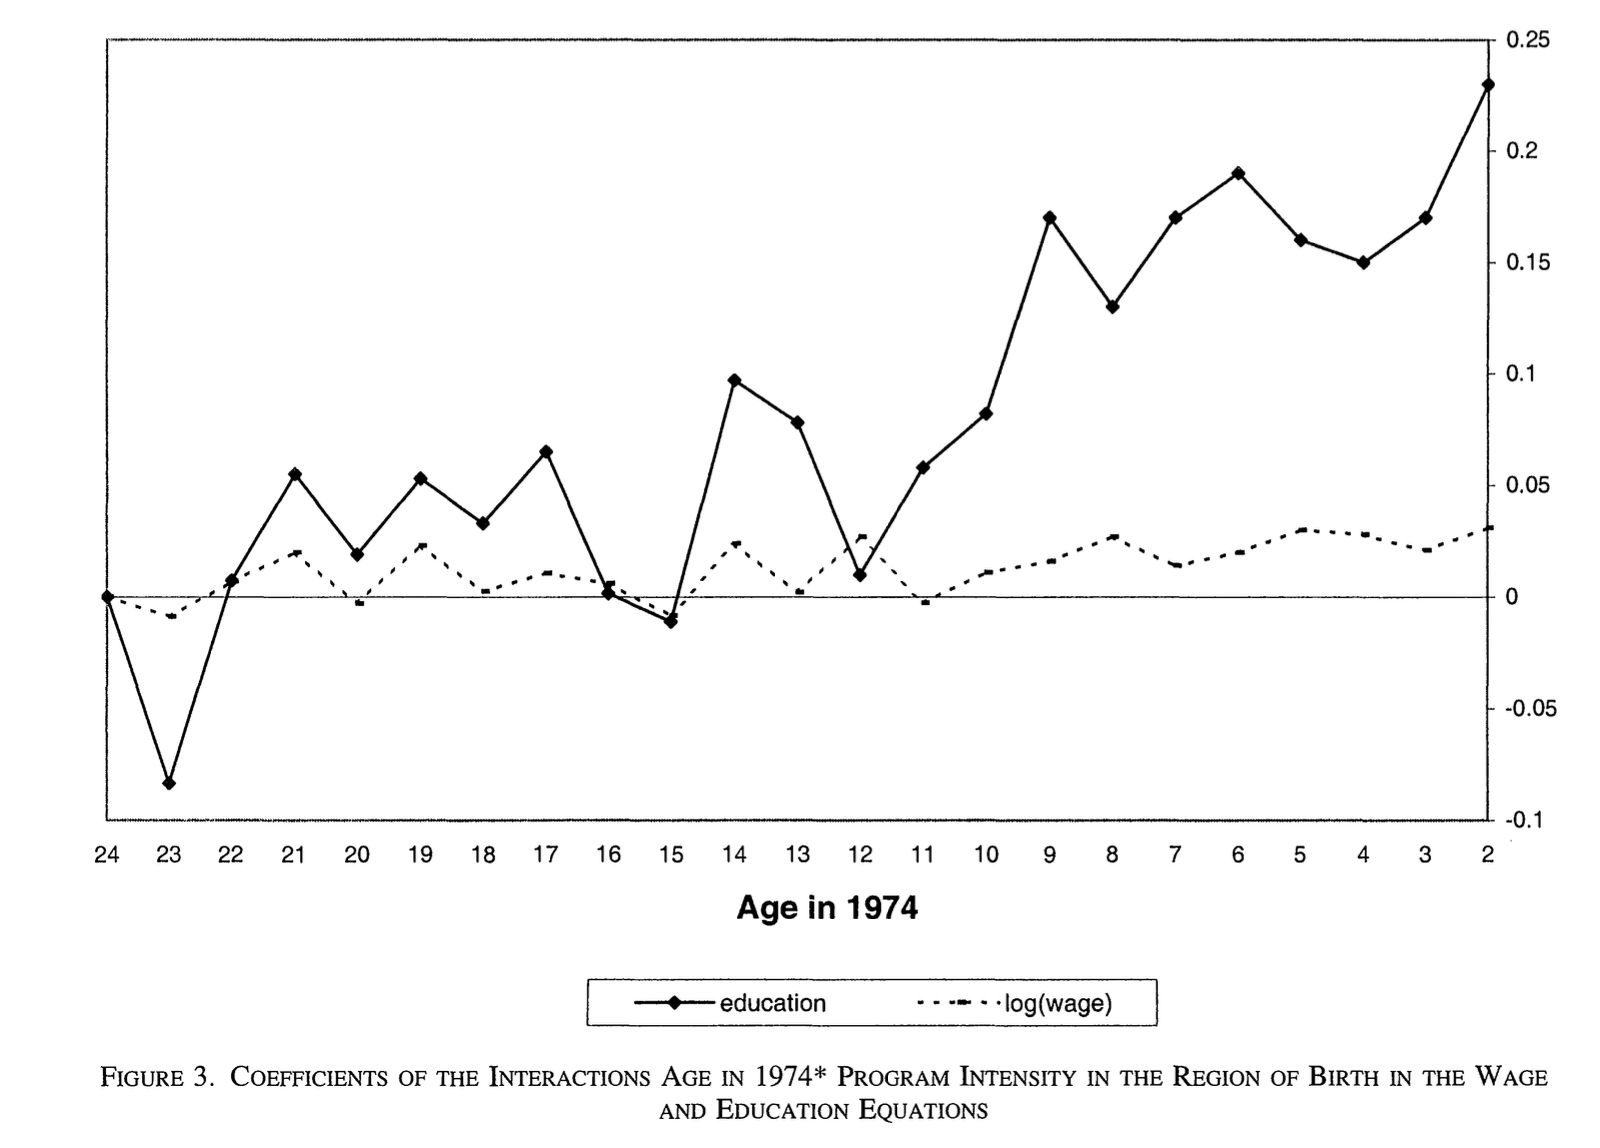
\includegraphics[width=0.4\textwidth]{inputs/Figure3.png}
\end{figure}
\end{frame}
%---------------------------------------------------------------------


%---------------------------------------------------------------------
\begin{frame}{Results (VIII)}
\begin{itemize}
\item Here are the main results of the paper
\item Returns to education around 7\%
\end{itemize}
\begin{figure}
    \centering
    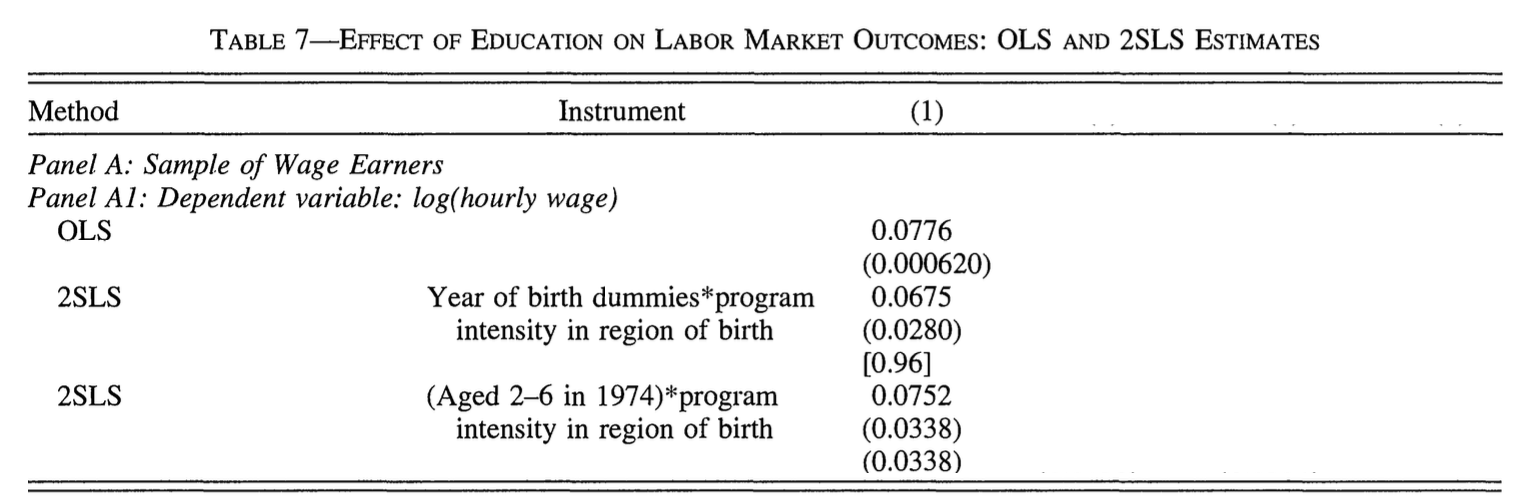
\includegraphics[width=\textwidth]{inputs/Table7.png}
\end{figure}
\end{frame}
%---------------------------------------------------------------------

%---------------------------------------------------------------------
\begin{frame}{Cost-Benefit Analysis}
\begin{itemize}
\item The paper ends by comparing INPRES's impacts to its costs
\item Three big assumptions author needs to make:
\begin{itemize}
    \item  How big is the dead-weight burden of taxes?  \textbf{Assumes 0.2-0.6 for each unit of tax}
    \item  Does schooling increase earnings by increasing productivity or by signalling/rent capture?  \textbf{Assumes the former}
    \item  Externalities of education? Assumes none
\end{itemize}
\item  Benefit of INPRES, in each year, is $\alpha\times GDP \times S\times\ E$
\item $\alpha$ is the labour share of GDP, $S$ is the share of wages earned by cohort that benefits from INPRES and $E$ is the estimated average effect of the program
\item  Estimates costs of building and running INPRES schools
\item  Finds that INPRES had an internal rate of return between 9\% and 12\%
\begin{itemize}
    \item Higher than the interest rate of Indonesia's sovereign debt at the time
    \item So it's profitable to fund more school building with government debt
\end{itemize}
\end{itemize}
\end{frame}
%---------------------------------------------------------------------

%---------------------------------------------------------------------
\begin{frame}{Conclusion}
\begin{itemize}
\item INPRES leads to more schooling and more earnings
\item If we use exposure to INPRES (within region) as an IV, we obtain returns to education around 5-10\%
\begin{itemize}
    \item In line with a large literature, including the seminal Angrist \& Krueger (1991) paper
\end{itemize}
\item But there are a few problems with this 
\begin{itemize}
    \item INPRES did more than just school building
    \item Poor regions may catch up with rich regions independently of INPRES
    \item Negative spillovers and general equilibrium effects? Impacts on broader labour markets due to stock of educated workers?
\end{itemize}
\end{itemize}
\end{frame}
%---------------------------------------------------------------------

\section*{Problem Set 2}

%---------------------------------------------------------------------
\begin{frame}{Comments}
\begin{itemize}
    \item When discussing spillover effects from an RCT intervention into the control group:
    \begin{itemize}
        \item It's not that the intervention becomes less effective - it could be more effective depending on the type of spillover
        \item Estimates are biased towards zero if we are (incorrectly) assuming that the control group is not exposed to treatment
    \end{itemize}
    \item Creating categorical variables in Stata, generating numeric variables
    \item Important note: for the control group, even though the beneficiary variable is missing, make sure you assign it a value of zero for the indicator mother or father variables. 
\end{itemize}
\end{frame}
%---------------------------------------------------------------------




%---------------------------------------------------------------------
\begin{frame}
\begin{center}{\LARGE See you next time!}\end{center}
\end{frame}
%---------------------------------------------------------------------


\end{document}
